% !TEX root = ../../thesis.tex
%______________________________________________________________________________
%
% SECTION
\section{Cut Cells}
\label{section:cutcells}
%
%______________________________________________________________________________

What is the significance of cut cells?
What are the issues with them?
What are the options to handle them in the SCM?
Touch on badly cut cells too!

Cells that are inside the physical domain in their entirety are treated identically as in the SEM, while others located completely in the fictitious domain can be discarded. However, the main issue of the SCM arises when dealing with cells that have points in both domains (cut cells).

While adaptive integration schemes can be used to accurately compute the element stiffness matrices $\mathbf K^e$ and load vectors $\mathbf f^e$, mass matrices $\mathbf M^e$ do not have this option. Adaptive integration introduces new quadrature points that do not coincide with the Gauss-Lobatto points, leading to non-zero off-diagonal entries in the mass matrix. However, standard Gauss-Lobatto quadrature is unsuitable for integrating discontinuous functions. The two possible approaches to solving this problem are:

\begin{itemize}
	\item finding an integration scheme capable of dealing with discontinuities while preserving the location of quadrature points
	\item diagonalizing mass matrices after integration
\end{itemize}

A candidate for the former is moment fitting, while the latter approach is covered by mass lumping schemes that have extensive literature.

%______________________________________________________________________________
%
% SECTION
\section{Moment Fitting}
\label{section:moment_fitting}
%
%______________________________________________________________________________

As described in \ref{subsection:moment_fitting}, moment fitting can be used to generate a quadrature scheme capable of integrating discontinuous functions while preserving a fixed set of integration points. At first glance, this makes it an excellent choice for handling cut cells in the SCM, however it's reduced accuracy renders it infeasible. To preserve the diagonality of the mass matrix, the polynomial order of the basis functions must uniquely define the integration order of the Gauss-Lobatto scheme $m=p+1$. Combined with the fact that the integrand of the mass matrix is of order $p_M=2p$, and that a quadrature scheme generated by moment fitting can only exactly integrate functions up to order $p_m^{MF}=m+1=p+2$ per direction, the integration error becomes too significant for this method to be viable.

In fact, this approach can lead to negative diagonal entries in the mass matrix even in simple cases, leading to a divergent solution in time. For example, a single square element cut half in figure \ref{fig:moment_fitting_cut_square}, with a basis of order 2 already yields such a mass matrix. With $\rho=1$ and $\beta=5$, the diagonal reads:

\begin{equation}
		[M_{ii}^e] =
		\begin{bmatrix}
			1.4^{-1} &
			2.2^{-1} &
			-2.8^{-2} &
			5.6^{-6} &
			8.9^{-6} &
			1.4^{-6} &
			2.2^{-6} &
			-2.8^{-7} \\
		\end{bmatrix}
\end{equation}

\begin{figure}[h]
	\centering
	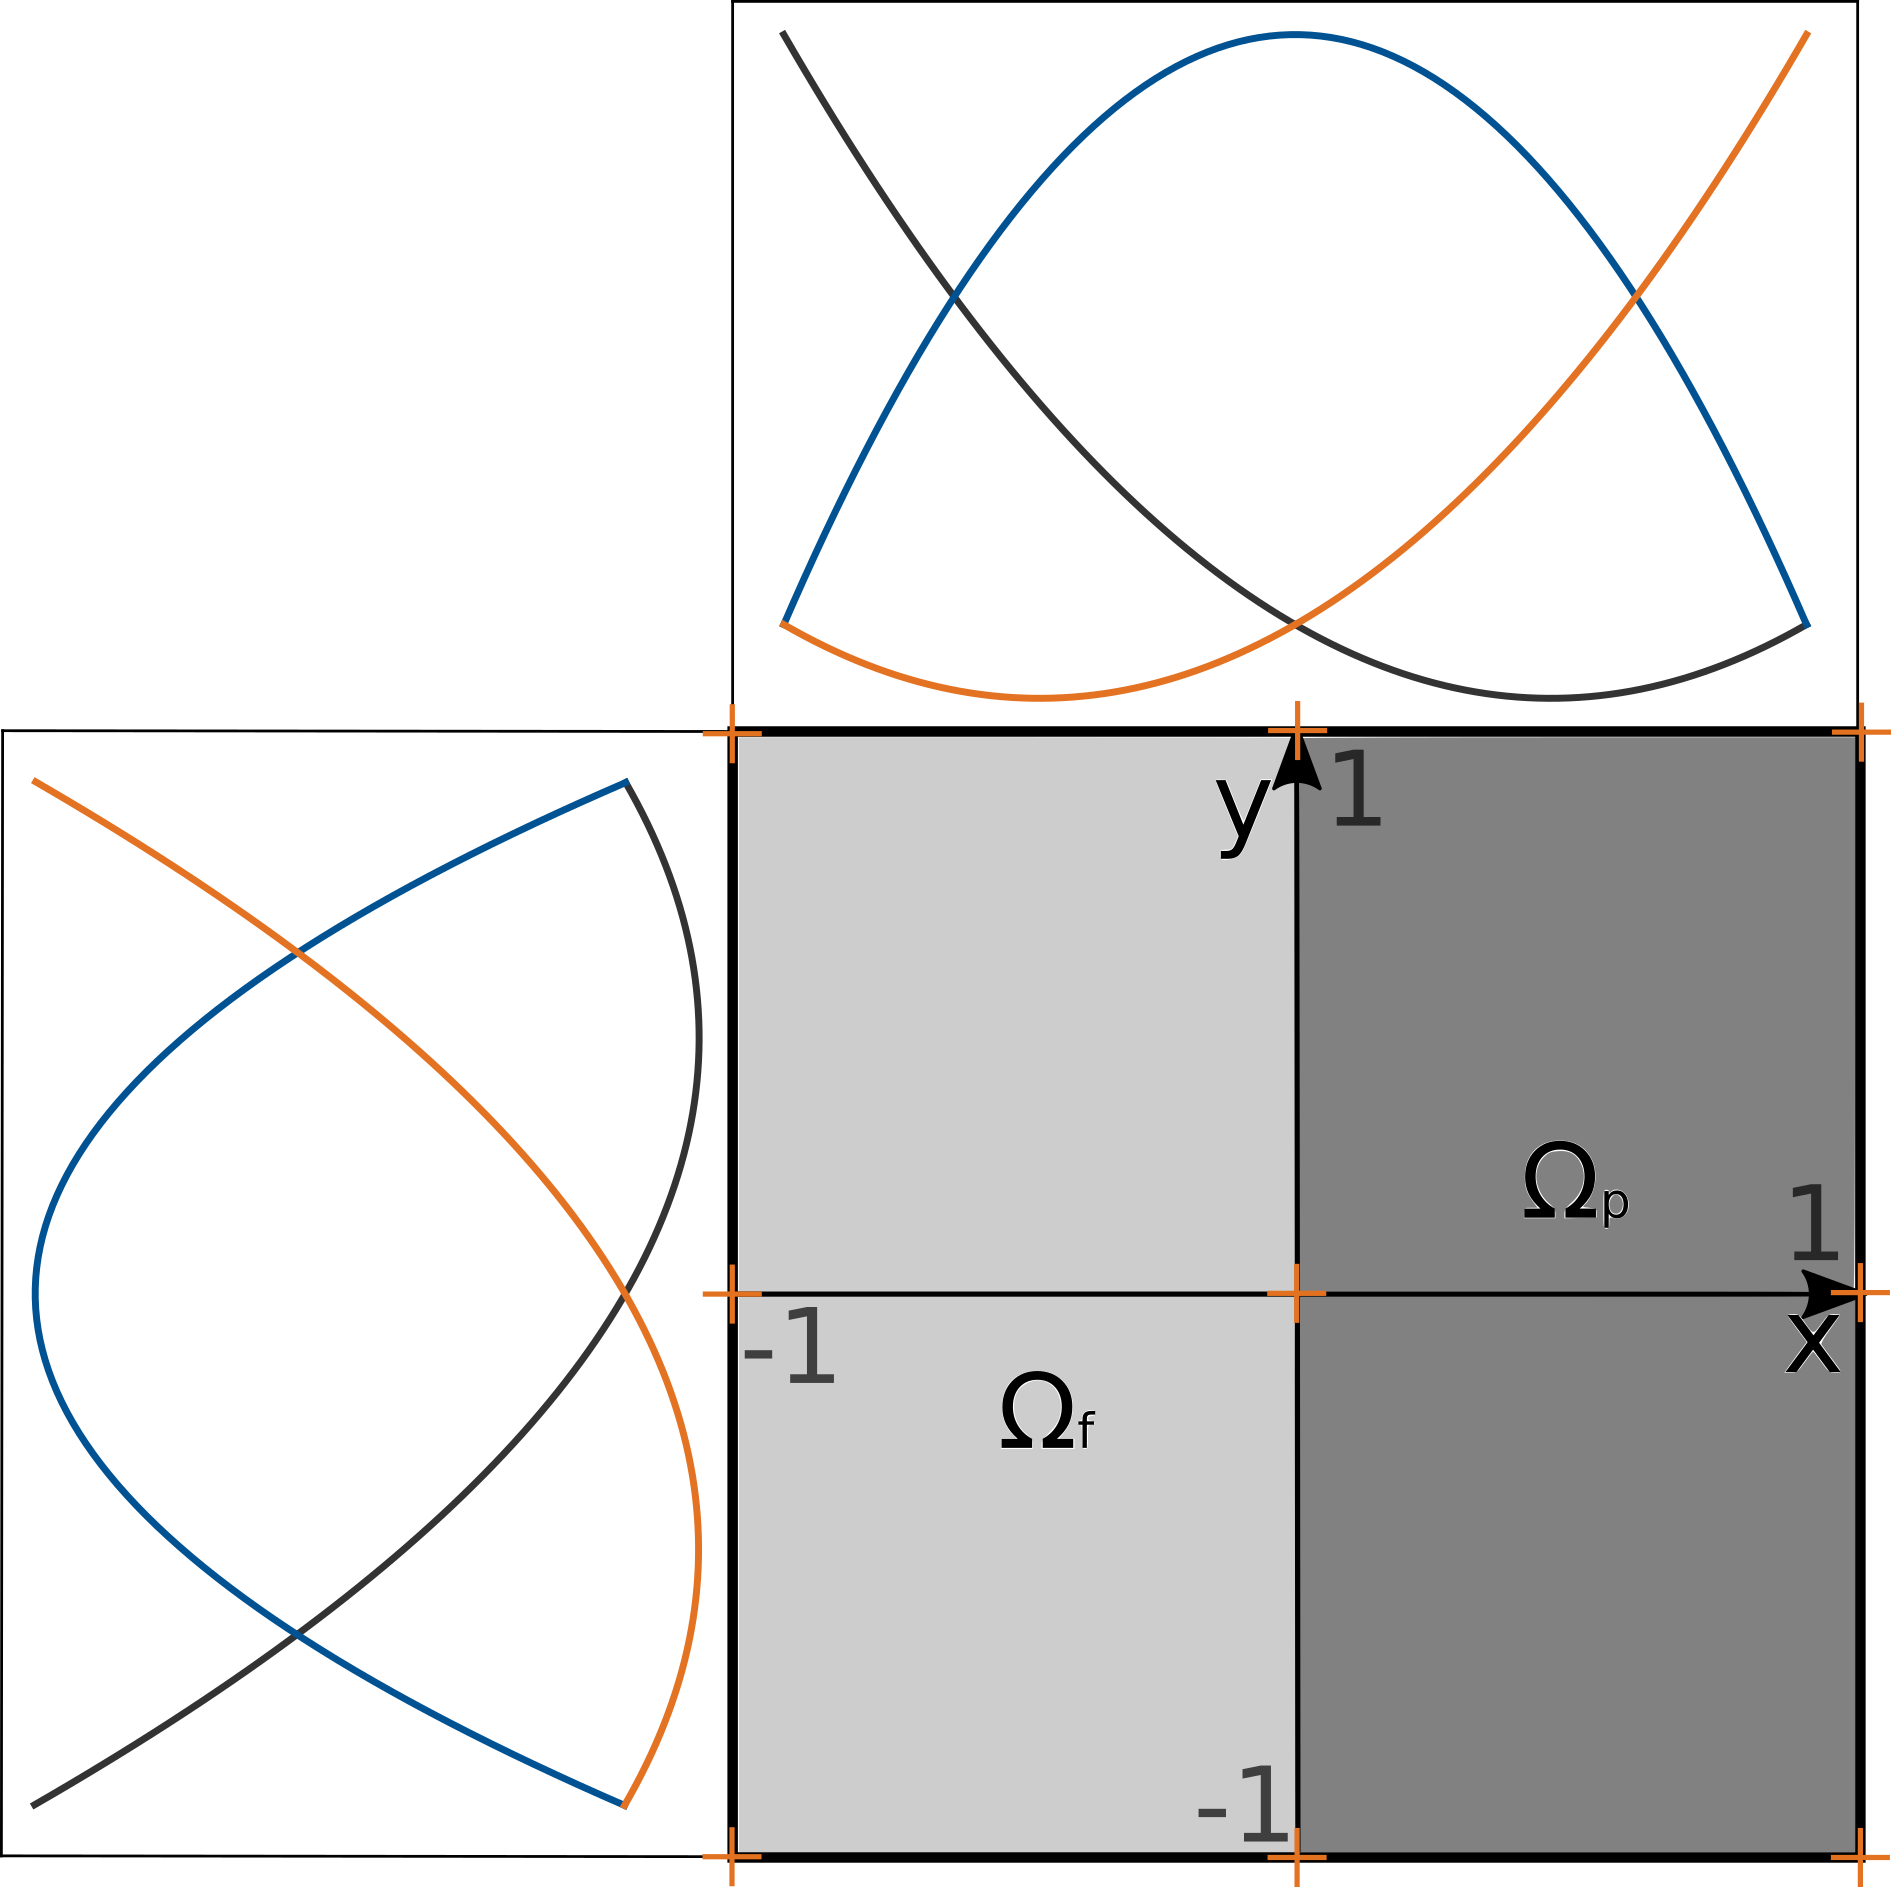
\includegraphics[height=7cm]{figures/moment_fitting_cut_square}
	\caption{Square cell cut in half along the $y$-axis with a Lagrange basis of order 2, and the corresponding Lobatto points.}
	\label{fig:moment_fitting_cut_square}
\end{figure}

Consequently, moment fitting cannot be used for the diagonalization of cut cells' mass matrices.